\chapter{Visualisierung der Koeffezienten sowie des Taylorpolynoms}

\begin{figure}[H]
    \vspace{-1em}
    \begin{center}
        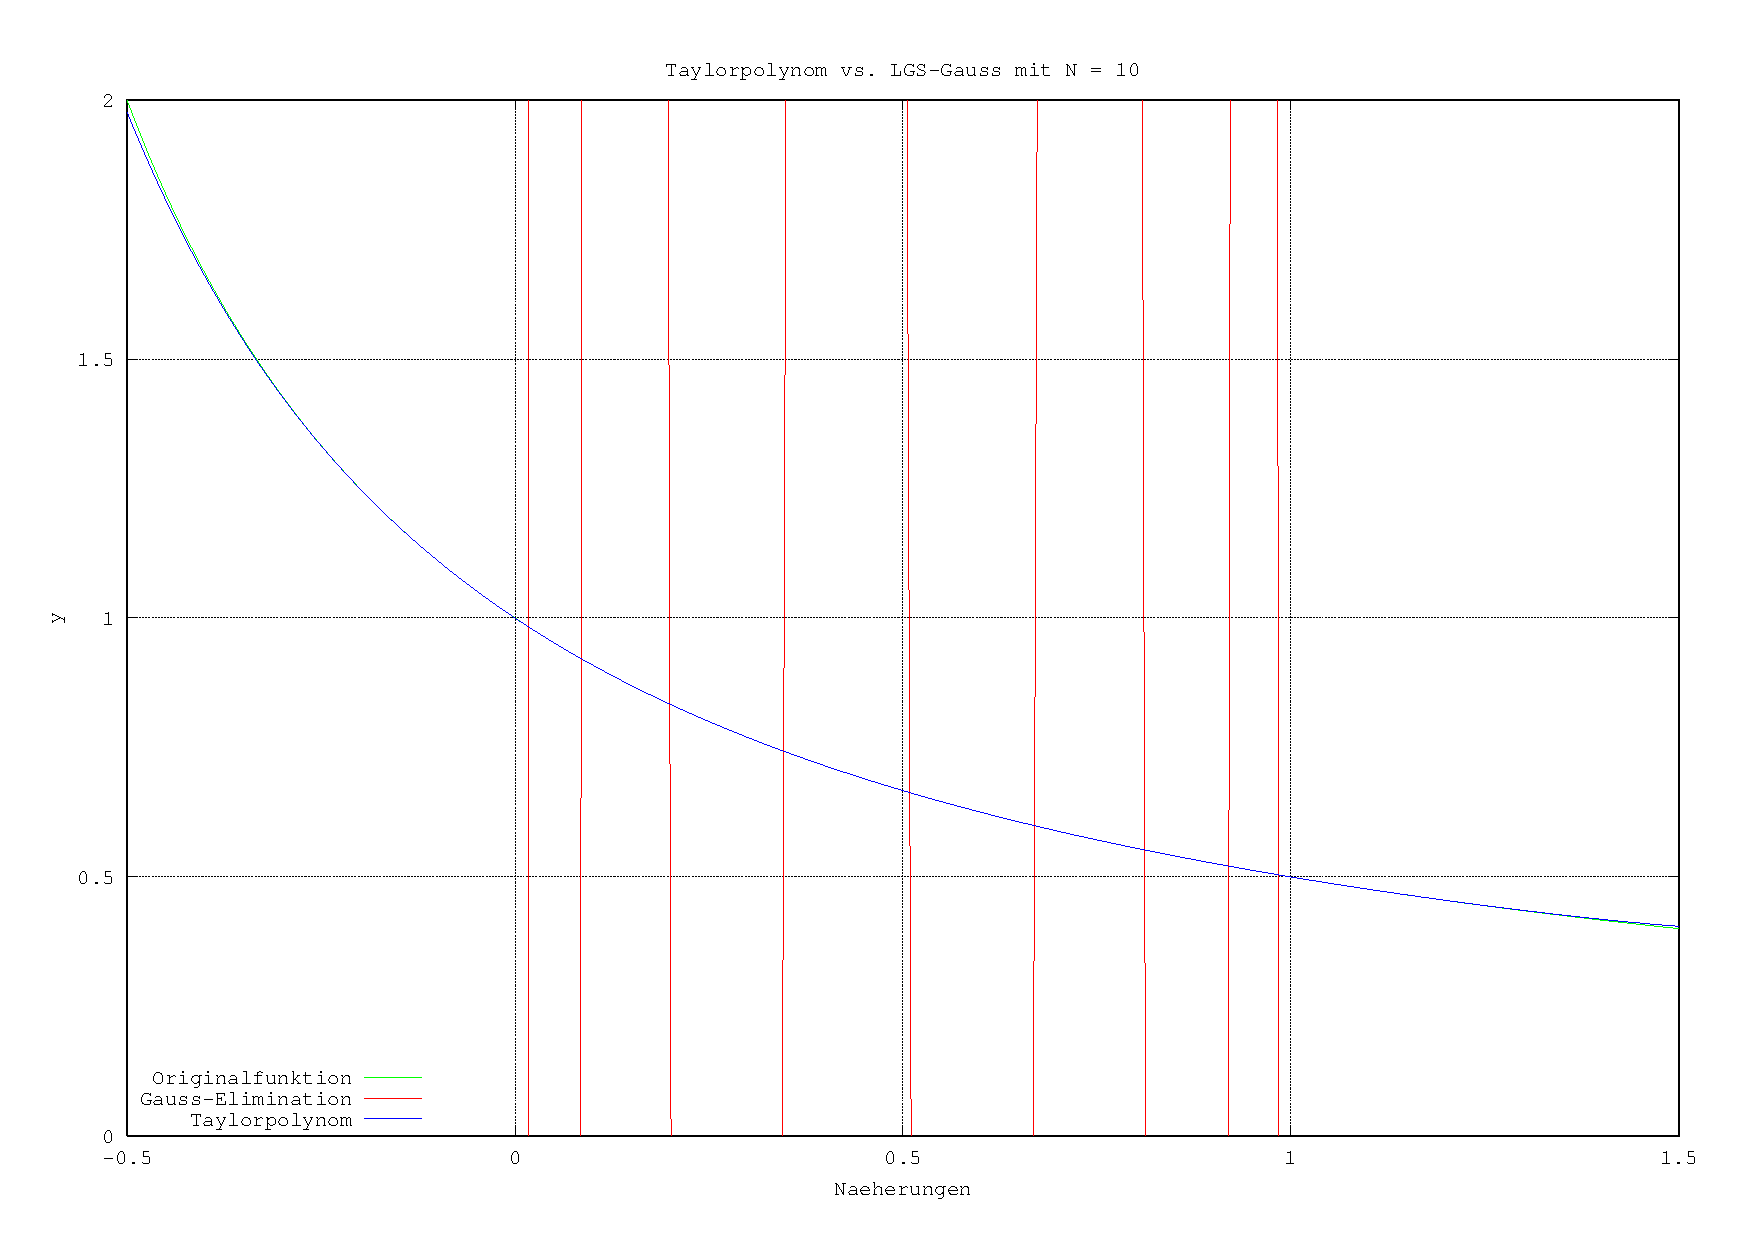
\includegraphics[width=\textwidth]{img/aufgabe5.pdf}
    \end{center}
    \vspace{-1em}
    \caption{Plot des Taylorpolynoms vs. Gauss-Elimination}
    \label{fig:TaylorVsGauss}
\end{figure}